\chapter{Context}

% As of today little work has been done on creating a multihop LoRa Network (see Kris Paper on RPL LoRa in context section)

\section{LoRa\label{section:lora}}

LoRa is a proprietary chirp spread spectrum technology made by Semtech with
integrated Forward Error Correction (FEC).
LoRa operate in this sub-GHz unlicensed Industrial, Scientific and Medical
(ISM) bands on multiple channels.
The main characteristics of LoRa, is that it trades data rate for long range 
and low power consumption with a maximum data rate of 27 kbps~\cite{8030482}.
LoRa supports bi-directional communications with maximum message length of 242
bytes~\cite{loraalliance:lorawanspecification}.

This section will cover the LoRa physical layer parameters, the packet structure and how
all these parameters influence the Time On Air (ToA).

\subsection{Chirp Spread Spectrum (CSS) modulation}

Chirp Spread Spectrum is a spread spectrum technique, developed in 1940 for
military application in radars and sonars \cite{semtech:modulationbasics}, but is 
getting adopted in the recent years for low power data transmission.
Chirp are sinusoidal signals increasing (upchirps) or decreasing (downchirps)
in frequency.
Fig~\ref{fig:downchirp} is an example of a downchirp.

Using CSS has the advantage to ensure equivalent timing and frequency offset
between the receiver and transmitter and robustness to channel degradation
mechanisms (multipath, fading, Doppler, in-band jamming
interference)~\cite{semtech:modulationbasics}.

\tikzset{declare function={f(\x)=sin(540*\x);}}

\begin{figure}[H]
\centering
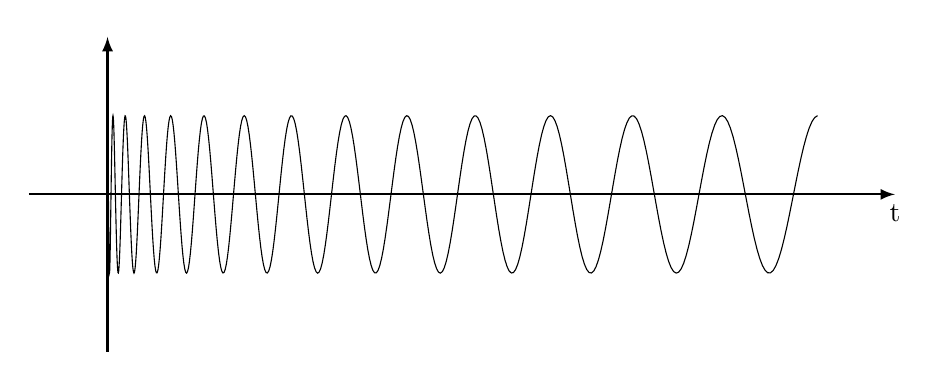
\begin{tikzpicture}
  \draw[thick,-latex] (0,-2) -- (0,2)node[right] {};
  \draw[thick,-latex] (-1,0) -- (10,0)node[below] {t};
  \draw[domain=0.1:9.5,variable=\x,samples=500] plot ({0.10*\x*\x}, {f(\x)});
\end{tikzpicture} 
\caption{Downchirp example\label{fig:downchirp}}
\end{figure}

\subsection{PHY Parameters}

\subsubsection{Spreading Factor (SF)}

The spreading factor, a parameter of the LoRa modulation, represent the
relation~(\ref{eq:sf}) between the symbols rate ($R_{s}$) and chirp rate ($R_{c}$)
(see~\cite{semtech:modemdesign}) where $2^{SF}$ equal to the number of chirps per
symbols.

\begin{equation}
 \label{eq:sf} 
  2^{SF} = \frac{R_s}{R_c}
\end{equation}

The SF can range from 7 to 12, higher SF improve the Signal-to-noise ratio
(SNR) and receiver sensitivity~\cite{semtech:modemdesign}.
Increasing the SF trade transmission range for slower communications.

The LoRa modulation uses orthogonal spreading factors to enable concurrent multiple
packet's transmission on the same channel with different
spreading factors~\cite{semtech:modulationbasics}.

\subsubsection{Bandwidth (BW)}

Bandwidth is the range of frequencies available during modulation.
LoRa support three bandwidth in the european ISM band.

\begin{itemize}
    \item 125 kHz
    \item 250 kHz
    \item 500 kHz
\end{itemize}

Available Bandwidth depends on the region. % See limit of lora wan
% Europe only use 125 and 250 kHz. source needed

The BW is interchangeable with the chirps rate, to do the symbols rate
calculation.
Increasing the BW increase the symbols rate, and thus, the data rate.

\begin{gather}
 \label{eq:bw} 
  BW = R_c (chips/s) \\
  R_s = \frac{BW}{2^{SF}} (symbols / sec)
\end{gather}

According to~\cite{semtech:modulationbasics}, increasing the
bandwidth increase the noise floor (\ref{eq:noisefloorbw}), reducing the
range of the communication.

\begin{equation}
 \label{eq:noisefloorbw} 
  Noise Floor = -174 + 10 \log_{10}(BW)
\end{equation}

% TODO Table with calculation

\begin{table}[h!]
\centering
\begin{tabular}{|c|c|}
\hline
\rowcolor[HTML]{C0C0C0} 
\multicolumn{1}{|c|}{\cellcolor[HTML]{C0C0C0}Bandwidth(kHz)} & Noise Floor (dBm) \\ \hline
125                                                          & -123              \\ \hline
250                                                          & -120              \\ \hline
500                                                          & -117              \\ \hline
\end{tabular}
\caption{Noise floor variation\label{table:bw}}
\end{table}


\subsubsection{Coding-Rate (CR)}

The Coding rate represent the proportion between information bit and error
correction bits. 
Forward Error Correction (FEC) is the process of adding error bits to a
transmission to help with data restoration in case of corruption.

Increasing the coding rate will decrease the data rate as communicating actual
information get longer but also more reliable.

The next table~\ref{table:cr} show the CR parameter available in LoRa.

\begin{table}[h!]
\centering
\begin{tabular}{|c|c|}
\hline
\rowcolor[HTML]{C0C0C0} 
  \multicolumn{1}{|c|}{\cellcolor[HTML]{C0C0C0}CR} & Proportion ($\frac{4}{4 + CR}$) \\ \hline
1                                                & $\frac{4}{5}$\\ \hline
2                                                & $\frac{4}{6}$\\ \hline
3                                                & $\frac{4}{7}$\\ \hline
4                                                & $\frac{4}{8}$\\ \hline
\end{tabular}
  \caption{Existing Coding Rates\label{table:cr}}
\end{table}

\subsubsection{Data Rate}

The following equation~\ref{eq:bitrate} calculate the bit rate depending on the
parameters I introduced in the previous sections\cite{semtech:modulationbasics}.

\begin{equation}
 \label{eq:bitrate} 
  R_{b} = SF \frac{\frac{4}{4 + CR}}{\frac{2^{SF}}{BW}} bits/sec
\end{equation}

The data rate can range from $0.3 kbps$ to $27 kbps$ depending on the \emph{SF} % TODO Calculation needed

% TODO datarange table

\subsection{Packet Structure}

This section covers the LoRa packet structure. LoRa employs two packet formats: 
the explicit mode and the implicit mode.
Three part constitute packets.

\begin{itemize}
  \item Preamble
  \item Optional Header
  \item Data payload
\end{itemize}

\begin{figure}[H]
  \centering
\begin{tikzpicture}[
  timeslot/.style={draw, rectangle, minimum size=1cm},
  description/.style={draw, rectangle, minimum size=1cm},
  arr/.style={help lines,black!70,<->},
]
\begin{scope}[xshift=0cm,yshift=0cm,inner sep=0pt, outer sep=0pt]
  \node (desc0) [description, fit={(0,0) (4,2)}, label=center:{Preamble}] {};
  \node (desc1) [description, fit={(4,0) (7,2)}, label=center:{Header}] {};
  \node (desc2) [description, fit={(7,0) (8,2)}, label=center:{CRC}] {};
  \node (desc4) [description, fit={(8,0) (13,2)}, label=center:{Payload}] {};
  \node (desc5) [description, fit={(13,0) (16,2)}, label=center:{Payload CRC}] {};
\end{scope}

\draw[arr]
  ([yshift=12pt]desc1.north west) -- node[fill=white] {$CR = \frac{4}{8}$} ([yshift=12pt]{desc2.north east});
\draw[arr]
  ([yshift=-10pt]desc1.south west) -- node[fill=white] {Explicit mode only} ([yshift=-10pt]{desc2.south east});

\draw[arr]
  ([yshift=12pt]desc4.north west) -- node[fill=white] {$CR$} ([yshift=12pt]{desc5.north east});
\end{tikzpicture}
\caption{LoRa Packet Structure\cite{semtech:sx}\label{fig:packetformat}}
\end{figure}

\begin{description}
  \item[Preamble] synchronize the receiver for the incoming data flow. The
    preamble length is configurable.
  \item[Header] Depend on the packet type explicit or implicit.
  \begin{description}
    \item[Explicit] mode header provides information on the payload.
    \begin{itemize}
      \item Payload length in bytes.
      \item Forward Error Correction code rate.
      \item The presence or not of the payload CRC.
    \end{itemize}
    \item[Implicit] mode remove the header from the packet. This mode should be
      used when payload, coding rate and CRC presence are known and we want to
      reduce the packet length.
  \end{description}
  \item[Payload] is a variable length field containing the transmitted data as
    well as an optional CRC.
\end{description}

\subsection{Time on Air (ToA)}

The Time on Air is the measure of packet transmission time.
ToA depends on the parameters we introduced previously to count the number of
symbols that constitute each communication of a payload.

The following formula define the duration of each symbol~\ref{eq:tsymlong}.
The equation~\ref{eq:tsym} is equivalent with the relation~\ref{eq:bw}.

\begin{equation}
  \label{eq:tsymlong}
  T_{sym} = \frac{1}{R_{sym}}
\end{equation}

\begin{equation}
  \label{eq:tsym}
  T_{sym} = \frac{2^{SF}}{BW}
\end{equation}

The ToA is the sum of the time to transmit the packet preamble and the packet
payload.

\begin{equation}
  \label{eq:tpacket}
  T_{packet} = T_{preamble} + T_{payload}
\end{equation}

The equation~\ref{eq:tpreamble} calculate the preamble time. The $n_{preamble}$
or preamble length is programmable.

\begin{equation}
  \label{eq:tpreamble}
  T_{preamble} = (n_{preamble} + 4.25)T_{sym}
\end{equation}

The following equation~\ref{eq:payloadsymnb} gives the number of symbols in the
payload of the packet.
The symbols number depend on the following parameters.

\begin{description}
  \item[PL] The payload length in bytes.
  \item[SF] The spreading factor.
  \item[H] Whether (0) or not (1) the header is enabled.
  \item[DE] Whether (1) or not (0) data rate optimization is enabled.
  \item[CR] The coding rate.
\end{description}

\begin{equation}
  \label{eq:payloadsymnb}
  n_{payload} = 8 + \max(ceil(\frac{8PL - 4SF + 28 + 16 - 20H}{4(SF - 2DE)})(CR + 4),0)
\end{equation}

The payload durations in~\ref{eq:tpayload} give the total packet time on air
with~\ref{eq:tpacket}.

\begin{equation}
  \label{eq:tpayload}
  T_{payload} = n_{payload} T_{sym}
\end{equation}


\subsection{Channels}

% See 'Understanding the limits of LoRaWAN' the 3 channels definition in Europe

\section{Time-Slotted Channel Hopping (TSCH)}

TSCH is a Medium Access Control (MAC) layer protocol defined by the IEEE
802.15.4 standard~\cite{rfc7554}.
The design inherited from WirelessHART and
ISA100.11a~\cite{Duquennoy2017TSCHA6}.
Time synchronization aim to achieve low power and highly reliable
communications by using the following principles.

\begin{description}
  \item[Time-division multiple access] or (TDMA) by assigning time-slots for each
    participant in the network avoiding collisions.
  \item[Synchronization] time-synchronized nodes syncing their clock with each
    other for improved power usage of the radio.
  \item[Channel Hopping] for better band usage, less interference and more
    throughput.
\end{description}

In the following section I will present the TSCH protocol building blocks.

\subsection{Time Slots}

Time slots are a fixed unit of time to execute the TSCH network operations. 
The duration of the time slot is not standardized and depend on the physical 
layer we are using. 
Time slots should be long enough for the longest frame size to be sent
between two nodes with an acknowledgement~\cite{rfc7554}. 
Every time slot in a TSCH network have the same duration.

For each time slots operations, a schedule orchestrate what each
node of the network will use his time-slot for.

\begin{description}
  \item [Transmit] if a packet is on the outgoing buffer of the node.
  \item [Receive] listen for incoming packets that may arrive.
  \item [Sleep]
\end{description}

\emph{Channel Hopping} increase the network capacity and multiple device can
share time-slots to transmit at the same time on different channels.

We can define \emph{links} as being made up of time slots and
channels~\cite{Chen2013PerformanceAO}.

\begin{equation}
  \label{eq:links}
  link = (TimeSlot_{number}, Channel_{offset})
\end{equation}

Multiple links constitute a time slot (dependent on the number of channel
available). Devices can transmit on different links during the same time slot.

\subsection{Slotframes}

Slotframes are a group of time slots that repeats over time as represented
in Fig~\ref{fig:timeslots}. 

The size of the slotframe will directly impact on the energy consumption of
each node as increasing the size will decrease the number of time a node has
to exit sleep mode to listen or transmit packets.

\begin{figure}[H]
  \centering

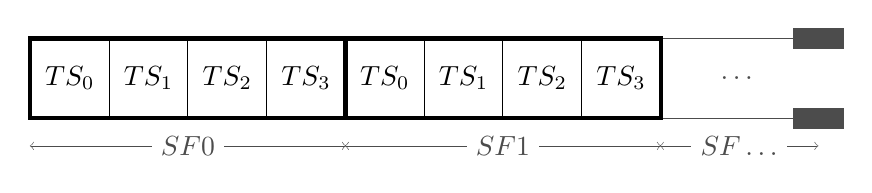
\begin{tikzpicture}[
  timeslot/.style={draw, rectangle, minimum size=1cm},
  arr/.style={help lines,black!70,<->},
]

\foreach [evaluate={\ts=int(mod(\i, 4))}] \i in {0,...,7} {
  \node (ts\i) [timeslot] at (\i, 0) {$TS_{\ts}$};
}
\node (ts8) [minimum height=1cm, minimum width=2cm, black!70] at (8.5, 0) {\ldots};
\draw[help lines, black!70]
  (ts8.north west) -- (ts8.north east) node[fill=white, black!70] {$\ldots$};
\draw[help lines, black!70]
  (ts8.south west) -- (ts8.south east) node[fill=white, black!70] {$\ldots$};

\draw[ultra thick] 
  (ts0.south west) rectangle (ts3.north east)
  (ts4.south west) rectangle (ts7.north east);

\draw[arr]
  ([yshift=-10pt]ts0.south west) -- node[fill=white] {$SF0$} ([yshift=-10pt]{ts3.south east});
\draw[arr]
  ([yshift=-10pt]ts4.south west) -- node[fill=white] {$SF1$} ([yshift=-10pt]{ts7.south east});
\draw[arr]
  ([yshift=-10pt]ts8.south west) -- node[fill=white] {$SF\ldots$} ([yshift=-10pt]{ts8.south east});

\end{tikzpicture}

\caption{Slotframes representation\label{fig:timeslots}}
\end{figure}


\subsection{Scheduling}

\subsection{Absolute Slot Number (ASN)}

ASN is a shared counter between all the devices that define the number of time slots 
elapsed since the start of the start of the network (see Fig~\ref{fig:asn}).
ASN increase after each time-slot and is calculated with \ref{eq:asn} where $k$
is the slotframe offset.

\begin{equation}
  \label{eq:asn}
  ASN = k SF_{len} + TS_{offset}
\end{equation}

\begin{figure}[H]
\centering
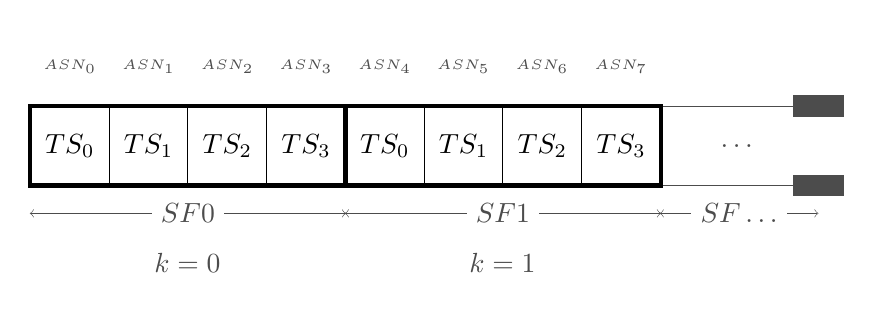
\begin{tikzpicture}[
  asn/.style={black!70, minimum size=1cm},
  timeslot/.style={draw, rectangle, minimum size=1cm},
  arr/.style={help lines,black!70,<->},
  desc/.style={black!70},
]

\foreach \i in {0,...,7} {
  \node (ts\i) [asn] at (\i, 1) {\tiny $ASN_{\i}$};
}
\foreach [evaluate={\ts=int(mod(\i, 4))}] \i in {0,...,7} {
  \node (ts\i) [timeslot] at (\i, 0) {$TS_{\ts}$};
}
\node (ts8) [minimum height=1cm, minimum width=2cm, black!70] at (8.5, 0) {\ldots};
\draw[help lines, black!70]
  (ts8.north west) -- (ts8.north east) node[fill=white, black!70] {$\ldots$};
\draw[help lines, black!70]
  (ts8.south west) -- (ts8.south east) node[fill=white, black!70] {$\ldots$};

\draw[ultra thick] 
  (ts0.south west) rectangle (ts3.north east)
  (ts4.south west) rectangle (ts7.north east);

\draw[arr]
  ([yshift=-10pt]ts0.south west) -- node[fill=white] {$SF0$} ([yshift=-10pt]{ts3.south east});
\draw[arr]
  ([yshift=-10pt]ts4.south west) -- node[fill=white] {$SF1$} ([yshift=-10pt]{ts7.south east});
\draw[arr]
  ([yshift=-10pt]ts8.south west) -- node[fill=white] {$SF\ldots$} ([yshift=-10pt]{ts8.south east});
\node[desc] at
  ([xshift=2cm, yshift=-28pt]ts0.south west) {$k = 0$};
\node[desc] at
  ([xshift=2cm, yshift=-28pt]ts4.south west) {$k = 1$};
\end{tikzpicture}
\caption{Absolute Slot Number\label{fig:asn}}
\end{figure}

\subsection{Channel Hopping}

\subsection{Network Formation}

\subsection{Synchronization}

\paragraph{Cost of the Synchronization}

% * Nodes are required to synchronize their time source periodically
% * It's highly dependant on the clock quality

\section{6LoWPAN}

% 6TOP Sublayer

\section{Contiki OS}

\section{Related work}

\subsection{Time-Slotted LoRa}

\subsection{Multihop LoRa}


